\documentclass[letterpaper,10pt]{memoir}

% === AUTOR === (((
\author{\textit{Por Erick I. Rodríguez Juárez.}}
% )))

% === PAQUETES === (((
% \usepackage{makeidx}
% \usepackage{xltxtra}
\usepackage{amsfonts}
\usepackage{amsmath}
\usepackage{amssymb}
% \usepackage{fullpage}
\usepackage{tikz}
\usetikzlibrary{arrows.meta}
\usepackage{graphicx}
% )))

% === TIPOGRAFÍA === (((
% \setmainfont[
  % BoldFont       = bodonibi,
	% ItalicFont     = Century modern italic2.ttf,
	% BoldItalicFont = bodonibi,
	% SmallCapsFont  = lmromancaps10-regular.otf
% ]{Century_modern.ttf}
% )))

% === COMANDOS === (((
% \newcommand{\dis}{\displaystyle}
% \newcommand{\qed}{\hspace{0.5cm}\rule{0.16cm}{0.4cm}}
% \newcommand{\operator}[1]{\mathop{\vphantom{\sum}\mathchoice
% {\vcenter{\hbox{\huge $#1$}}}
% {\vcenter{\hbox{\Large $#1$}}}{#1}{#1}}\displaylimits}
% \newcommand{\suma}{\operator{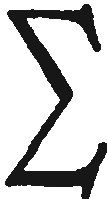
\includegraphics[scale=0.09]{FOTOS/Sigma.png}}}
% \setlength{\parindent}{0mm}
% )))

% === ITALICA EN ENTORNO MATEMÁTICO === (((
% \DeclareSymbolFont{italics}{\encodingdefault}{\rmdefault}{m}{it}
% \DeclareSymbolFontAlphabet{\mathit}{italics}
% \ExplSyntaxOn
% \int_step_inline:nnnn { `A } { 1 } { `Z }
 % {  \exp_args:Nf \DeclareMathSymbol{\char_generate:nn{#1}{11}}{\mathalpha}{italics}{#1} }
% \int_step_inline:nnnn { `a } { 1 } { `z } {  \exp_args:Nf \DeclareMathSymbol{\char_generate:nn{#1}{11}}{\mathalpha}{italics}{#1}}
% \ExplSyntaxOff
% )))

\begin{document}
	
\titulo

\begin{enumerate}
	\item Use \textbf{dfield} para dibujar el campo direccional respectivo, y traza a mano las curvas solución que pase por los puntos indicados.
		\begin{enumerate}
			\item \(\dfrac{dy}{dx} = \dfrac{x}{y}\), \(y(0) =5\), \(y(3) =3\), \(y(4) =2\), \(y(-5) =-3\).
			\item \(\dfrac{dy}{dx} =1-xy\), \(y(0) =0\), \(y(-1) =0\), \(y(2) =2\), \(y(0) =-4\).
		\end{enumerate}
	\item Use el método de las isóclinas para dibujar el campo direccional de 3 de las siguientes E.D. y esboza algunas soluciones de la E.D. incluyendo las soluciones de que satisfacen las condiciones dadas.\\[2mm]
		\begin{minipage}{0.5\linewidth}
			\begin{enumerate}
				\item \(\dfrac{dy}{dx}+y=3+ \dfrac{1}{x}\), \(y(1) =0\).
				\item \(\dfrac{dy}{dx} -y=0.2x^3\), \(y(0) = \dfrac{1}{2}\), \(y(2) =-1\).
				\item \(y \,' =y- \cos \dfrac{\pi}{2} x\), \(y(2) =2\), \(y(-1) =0\).
			\end{enumerate}
		\end{minipage}\hspace{5mm}
		\begin{minipage}{0.5\linewidth}
			\begin{enumerate}
			\setcounter{enumii}{3}
			\item \(\dfrac{dy}{dx} = \dfrac{1}{y}\), \(y(0) =1\), \(y(-2) =-1\).
			\item \(\dfrac{dy}{dx} =x^2+2y^2\), \(y(0) =1\).
			\item \(y \,' =y- \sin (\sin x)\), \(y(0) =0\).
			\end{enumerate}
		\end{minipage}
	\item Cada figura representa la gráfica de \(f(y)\) y \(f(x)\) respectivamente. A mano trace un campo de direcciones y algunas soluciones en una rejilla adecuada para \(y \,' =f(y)\), y \(y \,' =f(x)\). \\[2mm]
		\begin{minipage}{0.5\linewidth}
			(a)\\
			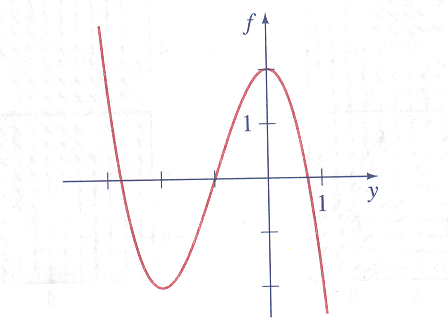
\includegraphics[width= 0.8 \linewidth]{IMAGENES/images/image19.png}
		\end{minipage}\hspace{5mm}
		\begin{minipage}{0.5\linewidth}
			(b)\\
			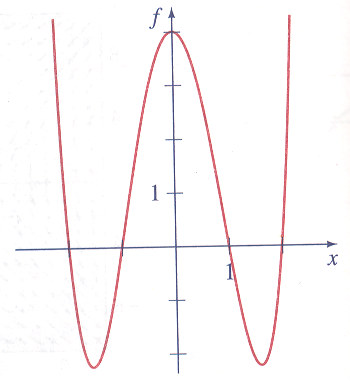
\includegraphics[width= 0.8 \linewidth]{IMAGENES/images/image21.png}
		\end{minipage}
	\item Elige 3 de las siguientes ecuaciones diferenciales autónomas. a) Determina sus puntos de equilibrio y clasifícalos usando la línea fase. b) Esboza algunas curvas solución con base a la información que nos da la tabla de características de monotonía y concavidad. Además, resalta la solución que satisface la condición inicial \(y(0) =1\).
		\begin{enumerate}
			\item \(y \,' -y^2+1=0\).
			\item \(\dfrac{dy}{dx} =10+3y-y^2\).
			\item \(y \,' =y^2(4-y^2)\).
			\item \(\dfrac{dy}{dx} - \cos y=0\).
			\item \(y \,' =y(y^2-2y-8)\).
		\end{enumerate}
	\item Para 2 las siguientes ecuaciones diferenciales, utilice la línea fase para predecir el comportamiento asintótico cuando \(t \longrightarrow \infty\) para la solución que satisface la condición inicial dada.
		\begin{enumerate}
			\item \(y \,' =2y^2(1-y^2)\), \(y(0) =0.5\).
			\item \(y \,' = y \ln (y+2)\), \(y(0) =1\).
			\item \(y \,' =y-y^3\), \(y(0) =1.1\).
		\end{enumerate}
\end{enumerate}
\textbf{NOTA:} : Revisa tu tarea con el software libre \texttt{dfield.jar} (\url{http://math.rice.edu/~dfield/dfpp.html})

\end{document}
